% !TEX program = xelatex
% SCU course-paper template adapted for this project; see THIRD_PARTY_NOTICES.md.
% Modified from supplied SCU course-paper template. Original licence preserved in ../LICENSE.
% Changes: English body labels, course title, long-name cover fitting.
% !TEX program = xelatex
% ============================================================
%  四川大学 · 研究生课程论文 LaTeX 模板
%  ----------------------------------------------------------
%  编译方式：XeLaTeX（Overleaf: Menu → Compiler 选 XeLaTeX；
%            本模板已附带 latexmkrc，Overleaf 通常会自动识别）
%  含参考文献的完整编译顺序：
%      xelatex → bibtex → xelatex → xelatex
%  排版规范改编自四川大学研究生学位论文模板 scuthesis2020
%  （https://github.com/kevinleeex/scu_thesis_2020，GPL 协议）
% ============================================================
\documentclass[a4paper,UTF8,zihao=-4,fontset=fandol]{ctexart}
% fontset=fandol：Overleaf / 任意系统免装中文字体即可编译；
% 本地 Windows 上如想用微软雅黑/宋体，可改为 fontset=windows。

% ---- 编译器保险：本模板只能用 XeLaTeX，误选 pdfLaTeX 时给出中文提示 ----
\usepackage{iftex}
\ifPDFTeX
  \PackageError{scu-course-paper}
    {本中文模板必须使用 XeLaTeX 编译，当前检测到的是 pdfLaTeX！\MessageBreak
     Overleaf：Menu -> Compiler -> 选择 XeLaTeX；\MessageBreak
     本地编译：使用命令 xelatex main.tex（不要用 pdflatex）}
    {切换编译器后重新编译即可。}
\fi

% ----------------- 封面 logo 开关 -----------------
\newif\ifcolorlogo
\colorlogotrue          % 彩色川大校徽；需要黑白版改为 \colorlogofalse

% ===================== 宏包 =====================
\usepackage{geometry}
\geometry{left=2.5cm,right=2.5cm,top=2.75cm,bottom=3cm,headsep=0.6cm,footskip=1cm}

\usepackage{graphicx}
\usepackage{caption}
\usepackage{subcaption}
\captionsetup{font=small,labelfont=bf,labelsep=quad}
\captionsetup[figure]{name=Figure}
\captionsetup[table]{name=Table}

\usepackage{amsmath,amssymb,amsfonts,amsthm,mathtools}
\usepackage{booktabs,longtable,multirow,array}
\usepackage{enumitem}
\setlist[itemize]{itemsep=2pt,parsep=0pt,topsep=4pt}
\setlist[enumerate]{itemsep=2pt,parsep=0pt,topsep=4pt}
\usepackage{float}

% 算法（中文标签）

\usepackage{xcolor}
% Unused TikZ illustration dependencies removed.

\usepackage{fancyhdr}
\usepackage[sort&compress]{gbt7714}   % GB/T 7714-2015 参考文献
\usepackage{hyperref}
\hypersetup{hidelinks}                % 打印友好，不显示链接彩色框；
                                      % 想要彩色链接可改为 colorlinks=true
\usepackage{cleveref}                 % 智能引用：\cref{fig:x} → 图 3-1

% 封面下划线（与学位论文模板同款；xeCJKfntef 仅 XeLaTeX 可用）
\ifXeTeX\usepackage{xeCJKfntef}\fi

% ===================== 基础格式 =====================
\linespread{1.5}                       % 1.5 倍行距
\setlength{\parindent}{2em}           % 首行缩进两字符
\setlength{\parskip}{2pt}
\setcounter{secnumdepth}{3}
\setcounter{tocdepth}{3}

% 图表、公式、定理、算法按“节”编号：图 1-1、式 (2-1)
\numberwithin{equation}{section}
\numberwithin{figure}{section}
\numberwithin{table}{section}
\renewcommand{\theequation}{\arabic{section}-\arabic{equation}}
\renewcommand{\thefigure}{\arabic{section}-\arabic{figure}}
\renewcommand{\thetable}{\arabic{section}-\arabic{table}}

% 定理类环境
\theoremstyle{plain}
\newtheorem{theorem}{定理}[section]
\newtheorem{lemma}[theorem]{引理}
\newtheorem{proposition}[theorem]{命题}
\newtheorem{corollary}[theorem]{推论}
\theoremstyle{definition}
\newtheorem{definition}[theorem]{定义}
\newtheorem{example}[theorem]{例}
\theoremstyle{remark}
\newtheorem{remark}[theorem]{注}
\renewcommand{\proofname}{证明}
\renewcommand{\thetheorem}{\arabic{section}-\arabic{theorem}}

% 各级标题：节（三号黑体居中）/ 小节（四号黑体）/ 小小节（小四黑体）
\ctexset{
  section/aftername={\hspace{\ccwd}},
  section={format=\centering\zihao{3}\heiti\bfseries,beforeskip=18pt,afterskip=18pt},
  subsection/aftername={\hspace{\ccwd}},
  subsection={format=\raggedright\zihao{4}\heiti\bfseries,beforeskip=18pt,afterskip=6pt},
  subsubsection/aftername={\hspace{\ccwd}},
  subsubsection={format=\raggedright\zihao{-4}\heiti\bfseries,beforeskip=12pt,afterskip=6pt},
  paragraph={format=\raggedright\zihao{-4}\kaishu,beforeskip=6pt,afterskip=0pt}
}
\renewcommand{\contentsname}{Contents}

% 页眉：《课程名称》课程论文；页脚居中页码
\makeatletter
\fancypagestyle{scuhead}{%
  \fancyhf{}%
  \fancyhead[C]{\zihao{-5}\songti 《\@coursename》课程论文}%
  \fancyfoot[C]{\zihao{-5}\songti\thepage}%
  \renewcommand{\headrulewidth}{0.8pt}}
\fancypagestyle{plain}{%
  \fancyhf{}%
  \fancyfoot[C]{\zihao{-5}\songti\thepage}%
  \renewcommand{\headrulewidth}{0pt}}
\makeatother
\pagestyle{scuhead}

% cleveref 中文引用名
\crefname{section}{节}{节}
\Crefname{section}{第}{节}
\crefname{figure}{图}{图}
\Crefname{figure}{图}{图}
\crefname{table}{表}{表}
\Crefname{table}{表}{表}
\crefname{equation}{式}{式}
\Crefname{equation}{式}{式}
\crefname{algorithm}{算法}{算法}
\Crefname{algorithm}{算法}{算法}
\creflabelformat{equation}{(#2#1#3)}

% ===================== 封面信息接口 =====================
\makeatletter
\newcommand{\papertype}[1]{\def\@papertype{#1}}
\newcommand{\coursename}[1]{\def\@coursename{#1}}
\newcommand{\papertitle}[1]{\def\@papertitle{#1}}
\newcommand{\college}[1]{\def\@college{#1}}
\newcommand{\majorname}[1]{\def\@majorname{#1}}
\newcommand{\studentname}[1]{\def\@studentname{#1}}
\newcommand{\studentid}[1]{\def\@studentid{#1}}
\newcommand{\teachername}[1]{\def\@teachername{#1}}
\newcommand{\termpaper}[1]{\def\@term{#1}}
\def\@papertype{研究生课程论文}
\def\@coursename{}
\def\@papertitle{}
\def\@college{}
\def\@majorname{}
\def\@studentname{}
\def\@studentid{}
\def\@teachername{}
\def\@term{}

% 封面填空下划线（与学位论文模板一致）
\newcommand{\fillinblank}[2]{%
  \CJKunderline[thickness=0.8pt,depth=0.45em]{\makebox[#1]{#2}}}

\newcommand{\makecover}{%
  \begin{titlepage}
    \thispagestyle{empty}
    \begin{center}
      \vspace*{-0.3cm}
      \ifcolorlogo
        
\includegraphics[width=9.2cm]{figures/SCU_TITLE.png}%
      \else
        
\includegraphics[width=9.2cm]{figures/SCU_TITLE_BW.png}%
      \fi
      \\[1.5cm]
      {\zihao{1}\heiti\bfseries \@papertype}
      \\[2.6cm]
      {\zihao{-3}
       \renewcommand{\arraystretch}{1.4}
       \begin{tabular}{@{}r@{\hspace{0.5em}}l@{}}
         {\heiti\makebox[2.8cm][s]{论文题目：}} & \fillinblank{7.4cm}{\songti\@papertitle}\\
         {\heiti\makebox[2.8cm][s]{课程名称：}} & \fillinblank{7.4cm}{\songti\@coursename}\\
         {\heiti\makebox[2.8cm][s]{学　　院：}} & \fillinblank{7.4cm}{\songti\@college}\\
         {\heiti\makebox[2.8cm][s]{专业名称：}} & \fillinblank{7.4cm}{\songti\@majorname}\\
         {\heiti\makebox[2.8cm][s]{学生姓名：}} & \fillinblank{7.4cm}{\songti\@studentname}\\
         {\heiti\makebox[2.8cm][s]{学　　号：}} & \fillinblank{7.4cm}{\songti\@studentid}\\
         {\heiti\makebox[2.8cm][s]{任课教师：}} & \fillinblank{7.4cm}{\songti\@teachername}\\
       \end{tabular}}
      \vfill
      {\zihao{4}\songti \@term}
      \vspace{1.0cm}
    \end{center}
  \end{titlepage}}
\makeatother


\setlength{\headheight}{16pt}
\emergencystretch=2em

\newcommand{\ComparisonText}{For the 0.5B model, executable feedback minus self-review is 0.0 percentage points (paired bootstrap 95\% interval 0.0 to 0.0). There are 0 improved and 0 regressed paired tasks. For the 1.5B model, executable feedback minus self-review is 0.0 percentage points (paired bootstrap 95\% interval 0.0 to 0.0). There are 0 improved and 0 regressed paired tasks. These descriptive intervals do not establish general equivalence or superiority. In a floor-effect condition, a zero-width empirical bootstrap interval reflects no observed successes in either branch, not certainty about unseen tasks.}
\newcommand{\LargeErrorText}{An exploratory decomposition for the 1.5B model finds correct numeric metric mappings on 0/24 initial, 0/24 self-review and 19/24 feedback-repair responses. This secondary diagnostic excludes units, row counts and chart fields and must not replace the primary correctness score. It helps distinguish arithmetic repair from complete-report repair. The field-level finding counts are preserved in \texttt{secondary\_diagnostics.json}.}

\papertype{课程论文}
\coursename{新型软件技术}
\papertitle{AI数据分析的可执行校验}
\college{}
\majorname{}
\studentname{\fontsize{10.5}{13}\selectfont BAHODIR KODIRJON UGLI NAZAROV}
\studentid{\small Omitted from public copy}
\teachername{胡大裟博士}
\termpaper{2026--2027 学年第 1 学期}
\begin{document}
\hypersetup{pageanchor=false}
\makecover
\hypersetup{pageanchor=true}
\thispagestyle{plain}
\section*{摘\hspace{1em}要}
大语言模型生成的数据分析可能同时包含计算错误、单位错误、有效样本数错误和图表数据不一致。
本文实现 TrustVerify，依据人工确认的分析契约，对结构化分析结果执行独立重算与逐字段校验。
系统支持六类描述性统计操作，并在无法支持的输入上拒绝给出校验结论。
实验区分受控错误注入与真实本地模型调用：前者用于检验校验层的覆盖范围，后者比较初始生成、
自我检查及可执行反馈修正。参考答案由独立的 SQLite 实现产生，生产校验器使用 Decimal 运算。
受控实验中，完整校验器检测到全部 288 个预设结构化错误，对 48 个正确报告未产生误报；
但全部 48 个仅含无依据因果叙述的报告仍通过结构化检查。真实模型实验中，1.5B 模型接受反馈后，
24 项任务中有 19 项的数值映射正确，但完整报告仍全部失败。该结果说明，通过数值与格式校验
不等同于整篇报告可信。本文同时公开模型原始响应、实验设置及复现代码，讨论契约错误、
叙述真实性、模型能力与小样本评估等限制。

\par\vspace{1em}
\noindent{\heiti 关键词：}大语言模型；数据分析；可执行校验；错误修正；可复现评估

\newpage
\section*{Abstract}
AI-generated analyses can contain arithmetic errors while presenting plausible prose.
TrustVerify recomputes six supported descriptive operations from a human-approved contract
and checks metric values, units, valid-row counts and chart data. We distinguish a controlled
mutation study from actual local-model generation. Sixty synthetic datasets provide 12
development and 48 test tasks, with an independent SQLite oracle. Across 336 injected faulty
reports, full verification detects 288 supported structured faults and misses all 48
unsupported causal narratives, with no false alarms on 48 clean reports. An actual-model
pilot compares initial generation, one self-review call and one executable-feedback repair
call on 24 paired tasks per model. The 0.5B model achieves no fully correct structured
reports in any generation condition. The 1.5B model also produces no fully correct reports, although executable feedback
corrects the numeric metric mapping on 19 of 24 tasks in an exploratory decomposition. Deterministic recomputation is sufficient for the approved contracts
and is reported separately from model improvement. The project contributes a working
prototype, field-level ablations, preserved raw calls and explicit reliability boundaries.
\par\vspace{1em}
\noindent\textbf{Keywords:} language models; data analysis; executable verification; feedback; reproducibility

\newpage{\small\linespread{1.05}\selectfont\tableofcontents}
\newpage
\section{Introduction}
Language models provide an accessible interface for data analysis, but a fluent explanation
does not establish that its calculations are correct. A report may use the wrong denominator,
count missing observations, attach a wrong unit, or plot values different from those in its
numeric result. These failures matter even in basic descriptive analysis. The central
engineering question is how much of a candidate analysis can be checked with executable
evidence and how precisely the resulting assurance should be described.

This project studies a bounded setting. A human approves the operation, columns, unit and
missing-value rule before verification. A model proposes a structured report. TrustVerify
recomputes the approved operation and returns field-specific findings. The model can then
receive those findings in one repair call. A separate deterministic path replaces the checked
fields directly. Neither path certifies free-form prose or discovers the correct research question.

Three research questions organize the study. RQ1 asks which error classes different checking
layers detect. RQ2 asks whether executable feedback improves structured correctness compared
with an equal-call self-review condition. RQ3 asks what role remains for the model when the
analysis contract is already explicit. The third question is essential: direct computation is
already sufficient for the six implemented operations. Any successful tool condition must
not be misrepresented as evidence that an LLM learned to reason more accurately.

The contributions are a dependency-free Python prototype, a reproducible synthetic benchmark
with an independent oracle, a controlled ablation, actual local-model response logs, and a
demonstration of both successful checks and failure boundaries. This is a course-scale
engineering and evaluation study. External feedback and arithmetic verification are established
ideas; the work does not claim a new general verification theory or a new language model.

\section{Related work}
\subsection{Evaluating data-science systems}
DSBench evaluates data-science agents on realistic tasks involving substantial files and
multi-stage analysis~\cite{jing2025dsbench}. It motivates examining observed outcomes rather
than treating generated analysis as completed work. Our synthetic benchmark has a different,
narrower purpose: exact control over the operation, missingness, source values and injected
fault. Results from this project are not directly comparable with DSBench scores and do not
measure end-to-end data-science competence.

\subsection{Self-review and external feedback}
Self-Refine studies iterative improvement using feedback from the same model without
additional model training~\cite{madaan2023selfrefine}. Its task-dependent results motivate
including a self-review baseline. Huang et al. investigate limitations of intrinsic
self-correction in reasoning~\cite{huang2024selfcorrect}. Their findings motivate an
independent computational signal, but do not establish that self-review always fails or
that every form of external feedback succeeds. This project evaluates those alternatives
under one explicit local protocol and preserves negative results.

\subsection{Local inference and structured reporting}
Qwen2.5 provides models of different capacities~\cite{qwen2024}. We use quantized 0.5B and
1.5B variants through Ollama's chat interface~\cite{ollama2026}. The experiment requests
JSON output but does not impose a strict JSON schema. Consequently, syntactically valid JSON
can still violate the report contract. These small local models make the study accessible,
but their results do not estimate the performance of larger hosted systems.

\section{Problem formulation}
\subsection{Approved contract and report}
Let $D$ be a CSV dataset, $C$ the human-approved contract and $R$ a candidate JSON report.
The contract specifies one of six operations, the required columns and the output unit.
The report contains a metric mapping, a unit string, an integer valid-row count, chart labels
and numeric values, and a narrative string. The verifier computes $E=f_C(D)$ and compares
the structured fields of $R$ with $E$.

For a scalar answer, the metric key is \texttt{value}. A grouped answer uses the group
labels as keys. Chart values must match their named metrics, although the chart label order
can vary. A field passes numeric comparison when
\begin{equation}
 |r-e|\leq\max\left(10^{-6},10^{-6}\max(|r|,|e|)\right).
\end{equation}
Booleans, numeric strings and non-finite values do not count as numeric answers. This
tolerance accommodates output rounding. It also defines a detectable-error boundary:
smaller differences can pass.

\subsection{Supported arithmetic}
The operations are sum, arithmetic mean, weighted mean, ratio of sums expressed as a
percentage, group sum and first-to-last percentage change. Weighted mean is
\begin{equation}
 \bar{x}_w=\frac{\sum_{i\in I}w_i x_i}{\sum_{i\in I}w_i},
\end{equation}
where $I$ includes rows with both values present. The percentage ratio is
\begin{equation}
 p=100\frac{\sum_{i\in I}x_i}{\sum_{i\in I}n_i}.
\end{equation}
It is deliberately defined as a ratio of sums, which differs from averaging row-wise
ratios. Percentage change uses the first and last nonmissing observations in CSV order.
The engine does not infer chronological order from column names.

Missing cells are excluded according to the columns required by the operation. All duplicate
records count as separate observations. The approved unit is used literally; dimensional
analysis is outside scope. Empty data, missing columns, unsupported operations, zero aggregate
denominators and invalid weights produce an abstention. The public API distinguishes
\texttt{pass}, \texttt{fail} and \texttt{abstain} so an unsupported task does not silently
receive a successful verdict.

\section{System design}
\subsection{Independent computation and field checks}
The production engine uses Python's Decimal arithmetic with a 40-digit calculation context
and emits finite JSON numbers. It never reads evaluation gold answers. The independent
evaluation oracle uses SQLite aggregation and separate query logic. Agreement between
these implementations checks common arithmetic mistakes, although it cannot eliminate
all shared specification errors.

The numeric profile checks metric labels and values. The schema-plus-numeric profile
also requires the expected top-level fields and selected field types. Full verification
adds unit equality, complete-case row count and chart consistency. These profiles provide
an ablation over coverage rather than three independently trained systems.

Each finding contains a code, field path, explanation and expected/observed values when
available. For example, an incorrect percentage can yield a finding for
\texttt{metrics.value} with the recomputed percentage. Such expected values are derived
from the available data and approved contract. They are computational feedback, not hidden
benchmark labels, but they do give the model more information than self-review receives.

\subsection{Repair paths and demonstration}
The model repair path receives the initial response and checker findings in one additional
call. The deterministic path recomputes the report without another model call. It replaces
the narrative with an explicit statement that no causal conclusion has been established.
We label this path deterministic recomputation throughout the results.

The local demonstration serves a task selector, an editable candidate report, the approved
contract and original rows. Users can inject a named fault, run an ablated checker and
recompute the structured report. All examples are visibly identified as controlled cases.
The application binds to loopback, accepts bounded JSON input and executes no submitted
Python or shell code. It is a local prototype, not a general code-execution sandbox.

\section{Experimental design}
\subsection{Datasets and split}
The generator creates ten datasets for each operation, using independently determined
seeds. Every dataset has 12 rows and three columns: numeric observation $x$, weight or
denominator $n$, and group $g$. Two observations of $x$ and one of $n$ are missing in
each dataset. Variants 00--01 form 12 development tasks, and 02--09 form 48 test tasks.
The model pilot uses variants 02--05, providing four test tasks per family and 24 per model.
Each task manifest includes a CSV SHA-256 digest.

This is a dataset-level split within six fixed task templates. It does not test transfer
to unseen operation families. All observations are synthetic and carry no substantive
claim about real people, institutions or economic outcomes.

\subsection{Controlled mutations}
For each of the 48 test tasks we retain a correct report and construct seven single-fault
reports. Six mutations target supported fields: a metric increased by 3.25, a wrong unit,
a valid-row count increased by one, a chart value increased by five, a missing chart and
a metric replaced by the string NaN. The seventh inserts an unsupported causal narrative
while preserving every structured value.

The resulting experiment contains 48 clean and 336 faulty reports, evaluated under each
profile. Mutation labels never enter the checker. Faults sharing one dataset are dependent,
and the types are intentionally chosen. Therefore, their detection proportions describe
coverage of the injected fault set, not the natural frequency or population prevalence of
LLM errors. We do not attach naive binomial confidence intervals to these mutation counts.

\subsection{Actual-model comparison}
The initial pilot uses Qwen2.5 0.5B. After observing frequent schema failures, we disclose a
capacity-check amendment and run Qwen2.5 1.5B on the same tasks with unchanged prompts.
This is a post-pilot capacity check rather than a preregistered independent replication.
Both models use temperature zero, seed 31415, context limit 4096 and a maximum of 384
generated tokens per call. Exact model digests, prompts and provider settings are saved.

For every task an initial call generates a report. Two separate branches then start from
that same initial report. One receives a self-review instruction with the data and question;
the other receives executable checker findings. Each branch gets exactly one additional
call with the same output-token limit. Thus each model contributes 72 calls: 24 initial,
24 self-review and 24 feedback repair. The branches have equal call count but differ in
prompt length and available computational information.

Invalid JSON or an invalid report is a measured content failure. Service/network failures
stop the run rather than being scored as model mistakes. Raw completed calls are retained,
and resuming a run checks request hashes. There is no content retry or selection of a
preferred response. Generated code is never executed.

\subsection{Metrics and uncertainty}
Primary correctness requires all metric labels/values, units, valid-row count and chart
data to match the independent oracle within tolerance. Narrative truth is excluded from
this metric. We also record JSON-object validity, field-level findings, wall-clock latency
and provider token counts. Model tables report cumulative initial-plus-second-call latency
for review and feedback. Deterministic computation time is reported separately.

We give Wilson 95\% intervals for each model condition and a task-level paired bootstrap
interval for feedback-minus-self-review accuracy, using 10,000 resamples and fixed seed
20261110. These intervals describe a small, clustered-by-template synthetic task sample.
They do not establish population-wide model performance or cross-model superiority.

\section{Results and error analysis}
\subsection{Checking layers and controlled coverage}
Numeric-only verification detects 96 of 336 injected faults (28.6\%). Requiring the report
schema increases detection to 144 (42.9\%). Full structured checking detects 288 (85.7\%).
All profiles produce zero false alarms on the 48 clean reports. Full verification detects
all 288 supported structured mutations, while missing all 48 causal-narrative mutations.
Figure~\ref{fig:coverage} shows the aggregate ablation and Figure~\ref{fig:matrix} separates
the fault categories.

\begin{figure}[H]\centering
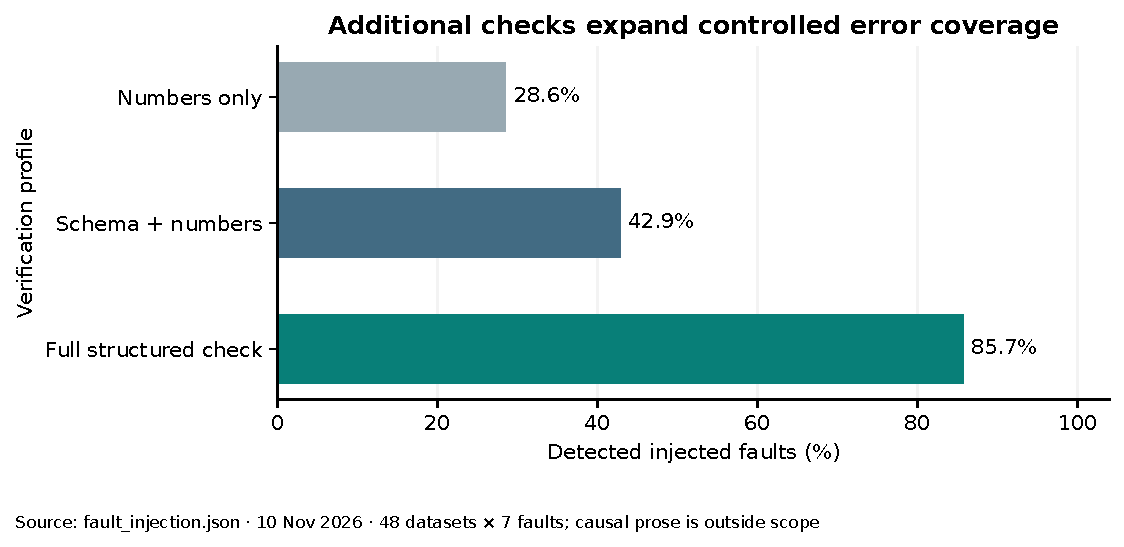
\includegraphics[width=0.97\textwidth]{figures/fault_coverage.pdf}
\caption{Detection of controlled injected faults. The denominator includes the intentionally
unsupported narrative mutation. These are checker-coverage results, not natural model error rates.}
\label{fig:coverage}\end{figure}
\begin{figure}[H]\centering
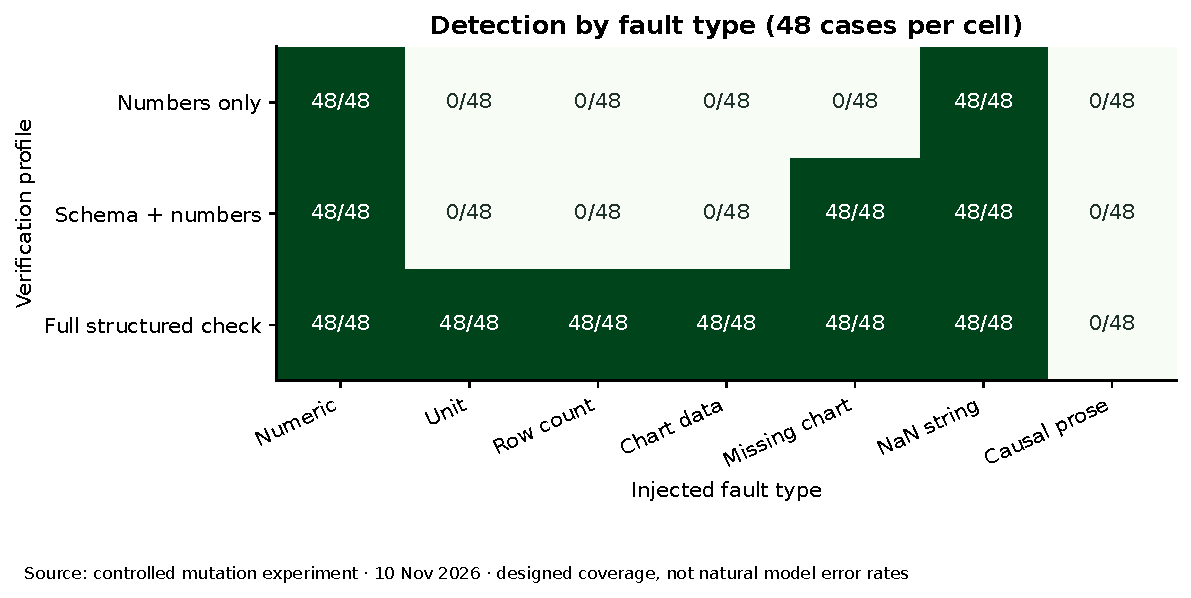
\includegraphics[width=0.98\textwidth]{figures/fault_matrix.pdf}
\caption{Detection counts by field and profile. Each cell contains 48 controlled cases.}
\label{fig:matrix}\end{figure}

This result is consistent with the design: numeric checking cannot discover a wrong unit
when the metric itself is unchanged. Schema checking can detect the missing chart but not
a present chart with wrong values. Full checking adds independent evidence for those fields.
However, because the mutations directly exercise designed checks, perfect supported-fault
detection is a coverage observation, not proof against arbitrary failures.

\subsection{Model outcomes}
\begin{table}[H]\centering\small
\caption{Measured actual-model pilot. Each generation condition uses 24 paired tasks.
Intervals are descriptive Wilson 95\% intervals for structured correctness.}
\label{tab:live}
\begin{tabular}{llrrr}
\toprule
Model & Condition & Correct & 95\% interval (\%) & Time (s) \\
\midrule
0.5B & Initial & 0/24 & 0.0--13.8 & 5.81 \\
0.5B & Self-review & 0/24 & 0.0--13.8 & 11.14 \\
0.5B & Feedback repair & 0/24 & 0.0--13.8 & 11.48 \\
1.5B & Initial & 0/24 & 0.0--13.8 & 7.08 \\
1.5B & Self-review & 0/24 & 0.0--13.8 & 14.14 \\
1.5B & Feedback repair & 0/24 & 0.0--13.8 & 15.29 \\
\bottomrule
\end{tabular}

\end{table}
\ComparisonText

\begin{figure}[H]\centering
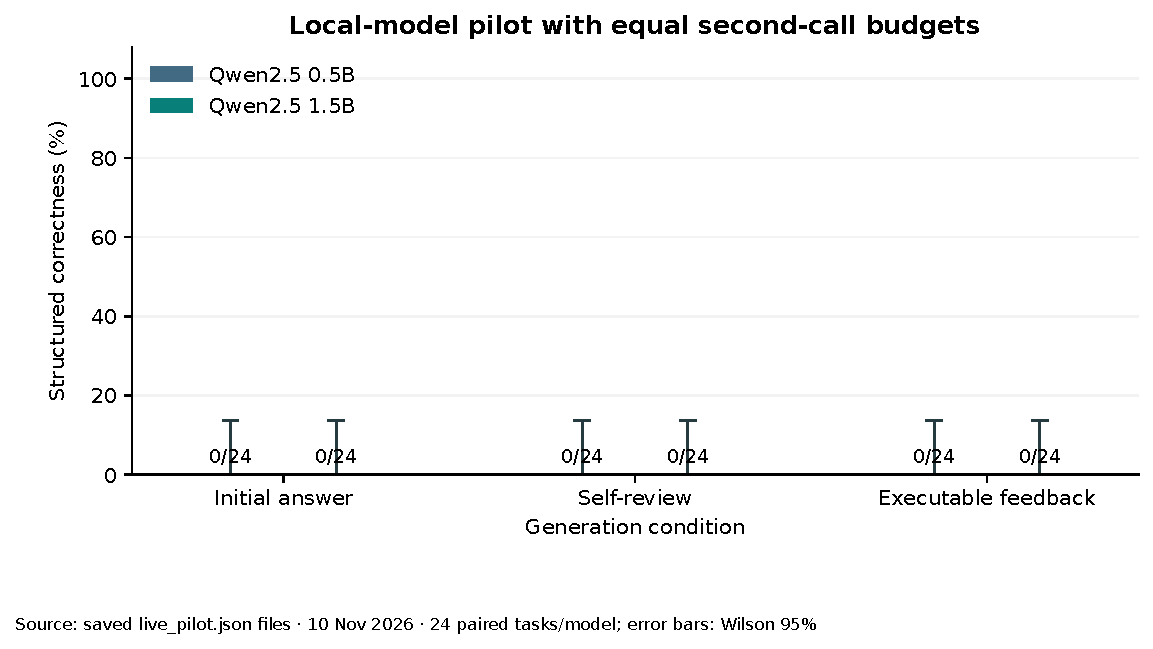
\includegraphics[width=0.98\textwidth]{figures/live_accuracy.pdf}
\caption{Observed structured correctness for actual local-model responses. Whiskers show
Wilson 95\% intervals. Deterministic recomputation scores 24/24 separately for each task set.}
\label{fig:live}\end{figure}

The 0.5B model produces JSON objects on 19 of 24 tasks in every generation condition, but
none satisfies the full structured correctness criterion. On task sum-02, it reports a value
of 10, embeds unit and row-count fields inside the metric mapping, and uses chart labels
that do not correspond to the expected single metric. Self-review and feedback repair
preserve these problems. This example illustrates that a parseable object is weaker than
a valid, correct report. The unchanged prompt and retained responses make this floor
effect visible instead of silently removing it from the evaluation.

\LargeErrorText

\subsection{What deterministic execution establishes}
Deterministic recomputation matches the independent oracle on all 60 generated tasks,
including all 48 held-out checker tasks and the 24-task pilot subset. This is an expected
consequence of correctly implementing an explicit operation. It provides a useful
deployment path for supported contracts, but does not constitute language-model reasoning
improvement. It also makes the project's arithmetic boundary clear: when the operation is
known, conventional software is the appropriate source of the result.

The model may still be useful for proposing a readable interface or a narrative, but those
roles require additional validation. Our reported correctness metric cannot evaluate them.
It would be misleading to translate 24/24 deterministic accuracy into a claim that the
entire assistant is fully reliable.

\section{Threats to validity and limitations}
\subsection{Internal validity}
Using Decimal and SQLite reduces identical-implementation bias, but both follow the same
written contract. A wrong contract can make both implementations agree on the wrong task.
Likewise, final scoring shares a numeric-tolerance policy with checking. Hand-calculated
unit tests provide an additional independent check for representative operations.

The feedback branch receives expected values computed from the data, while self-review
does not. Consequently, the experiment compares complete systems with different evidence
access. Equal generation counts do not make available information, token counts or total
computation identical. Cold-start loading, caching and hardware scheduling affect measured
latency. Wall-clock results are local observations, not general speed benchmarks.

\subsection{Construct and external validity}
Structured correctness excludes narrative accuracy, causal validity, input-data quality,
visual chart design and choice of statistical method. In the causal-claim mutation, all
structured fields can pass while the report makes an unjustified assertion. In a second
scope challenge, changing an approved sum contract to a mean contract and computing that
mean correctly also passes. The verifier has no evidence of the user's original intent.

The synthetic tasks are small, have fixed templates and cover only six descriptive
operations. Two small quantized models and one generation seed offer limited generalization.
The larger model was selected after inspecting the smaller pilot, which we disclose.
Bootstrap uncertainty over 24 tasks does not account for all model, dataset, hardware or
prompt variation. Wider evaluations should add independently sourced real datasets,
unseen task families and stronger models while retaining these original results.

\subsection{Practical assurance}
A pass should read ``checked structured fields agree with this approved contract'', never
``the report is true''. Unsupported tasks should route to human review. A practical extension
would ask a user to approve the proposed contract and inspect data-quality decisions before
generation. Free-text claims could receive a separate, calibrated evidence review. These
extensions are future work and have not been implemented or evaluated here.

\section{Reproducibility and software quality}
The core package uses Python 3.10 or later with no third-party runtime dependencies.
The repository includes 60 CSVs, their task manifests and hashes, independent oracle values,
controlled fault records, model-call logs, summary statistics, figure source and the report
source. Tests cover hand calculations, missingness, undefined contracts, malformed reports,
chart consistency, repair behavior, known blind spots and oracle agreement.

The main reproduction commands are listed below. They run from the repository root.
\begin{quote}\small\ttfamily
python3 -m unittest discover -s tests -v\\
python3 -m trustverify.cli generate\\
python3 -m trustverify.cli benchmark\\
python3 scripts/check\_results.py\\
python3 -m trustverify.server
\end{quote}
The first command runs the tests, the second regenerates data, the third reproduces
controlled results, the fourth checks saved model evidence without new calls, and the
last starts the demonstration. The README gives full model and manuscript instructions.

The report adapts the supplied SCU format, preserving A4 geometry, bilingual abstracts,
section numbering and GB/T 7714 references. The supplied licence file is AGPL-3.0 despite
a GPL reference in its README; the original file and attribution are retained. Lecturer
slides are identified in a source manifest and are not redistributed.

\section{Conclusion}
TrustVerify provides executable evidence for a deliberately limited set of analysis claims.
The ablation shows how schema, unit, row-count and chart checks expand coverage beyond
numeric comparison. The causal-narrative and wrong-contract examples demonstrate why that
coverage cannot establish whole-report truth. In the 1.5B pilot, an exploratory decomposition finds that executable feedback produces
19/24 correct numeric mappings, compared with 0/24 for self-review, while full-report
correctness remains 0/24 in both branches. The actual-model comparison therefore exposes
the gap between arithmetic repair and complete-report compliance. The deterministic
baseline shows that conventional computation already solves approved descriptive contracts.
The practical outcome is a reproducible checking tool with inspectable failure boundaries.

\paragraph{AI assistance and author responsibility}
Codex assisted with implementation, experiment execution, drafting and layout. Reported
model outputs are preserved local Ollama calls; controlled errors are synthetic. The author
must reproduce and understand the work before submission. No instructor approval or grade
is claimed.

\clearpage
{\zihao{5}\bibliographystyle{gbt7714-numerical}\bibliography{refs}}
\end{document}
